\documentclass[12pt,a4paper,preprint,nopreprintline]{elsarticle}

\usepackage[T2A]{fontenc}
\usepackage[utf8]{inputenc}
\usepackage[russian]{babel}
\usepackage{amsmath,amssymb,amsfonts,bm}
\usepackage{graphicx}
\usepackage{booktabs}
\usepackage{multirow}
\usepackage{array}
\usepackage{tabularx}
\usepackage{xcolor}
\usepackage{hyperref}
\graphicspath{{figs/}}

\usepackage[
    a4paper,
    left=2cm,
    right=2cm,
    top=2cm,
    bottom=2.7cm
]{geometry}

% На страницах с плавающими объектами прижимаем содержимое к верхнему краю.
\makeatletter
\setlength{\@fptop}{0pt}
\setlength{\@fpsep}{8pt}
\setlength{\@fpbot}{0pt plus 1fil}
\makeatother
\setlength{\abovecaptionskip}{4pt}
\setlength{\belowcaptionskip}{2pt}
\renewcommand{\floatpagefraction}{0.05}

\begin{document}
\makeatletter
\setlength{\@fptop}{0pt}%
\setlength{\@fpsep}{8pt}%
\setlength{\@fpbot}{0pt plus 1fil}%
\makeatother

\begin{frontmatter}

\title{Спектр возмущений течения Мишеля:\\
акустические, вихревые и энтропийные моды}

\author{Alexander V. Semyannikov}
\ead{avsemyannikov@gmail.com}
\address{Independent Researcher}

\begin{abstract}
Мы исследуем спектр линейных возмущений релятивистской сферической аккреции на чёрную дыру Шварцшильда (течения Мишеля), перенося на полную общую относительность ньютоновский анализ пространственной устойчивости аккреции Бонди. Малые возмущения идеальной жидкости разделяются на три семейства -- акустические, вихревые и энтропийные моды, -- которые мы рассматриваем совместно на языке акустической геометрии. Акустический сектор сводится к одномерному уравнению шрёдингеровского типа с явным эффективным потенциалом: в вакуумном пределе оно воспроизводит стандартный скалярный потенциал Шварцшильда, а в нерелятивистском -- известное ньютоновское волновое уравнение течения Бонди. Для трансзвукового фона Мишеля звуковая точка в точности совпадает с акустическим горизонтом, и анализ Фробениуса показывает, что этот горизонт заменяет ньютоновский центральный конец области: нетривиальный радиальный показатель чисто мнимый, так что локальные решения представляют собой бегущие волны, а не растущие степени. Главный результат состоит в том, что акустический горизонт регуляризует внешнюю пространственную задачу. Ньютоновская нерадиальная неустойчивость, работающая при $\gamma<5/3$, опирается на рост возмущения к концу области в точечной массе; во внешней области Мишеля такого конца нет -- относительные амплитуды всех трёх секторов выходят у горизонта на конечные значения, -- а сверхзвуковая оболочка причинно от неё отделена. Вихревые и энтропийные возмущения являются адвективными инвариантами с единственной входящей характеристикой: будучи вморожены в поток, они сносятся сквозь горизонт, а энтропийная мода вдобавок возбуждает звук и завихрённость через релятивистский бароклинный член. Численное интегрирование задачи рассеяния подтверждает сохранение потока и отсутствие сверхотражения. Тем самым внешне доступное течение свободно от ньютоновской центральной степенной неустойчивости.
\end{abstract}

\begin{keyword}
аккреция Мишеля \sep релятивистская гидродинамика \sep акустические возмущения \sep вихревые моды \sep энтропийные моды \sep пространственная устойчивость \sep акустический горизонт
\end{keyword}

\end{frontmatter}

\section{Введение}
\label{sec:introduction}

Стационарная сферическая аккреция представляет собой минимальную модель, в которой можно совместно исследовать гравитацию, сжимаемое течение и распространение волн. Её ньютоновская форма задаётся решением Бонди~\cite{BondiH_OnSphericallySymmetricalAccretion_1953}, а релятивистское течение на чёрную дыру Шварцшильда описывается решением Мишеля~\cite{MichelFC_AccretionOfMatterByCondensedObjects_1972}. Трансзвуковой фон обладает акустическим горизонтом, который управляет распространением линейных акустических возмущений и порождает эффективную релятивистскую акустическую геометрию~\cite{MoncriefV_StabilityOfStationarySphericalAccretionOntoASchwarzschildBlackHole_1980,BilicN_RelativisticAcousticGeometry_1999}.

Устойчивость стационарной сферической аккреции имеет долгую историю. В ньютоновской постановке течение Бонди устойчиво относительно радиальных возмущений~\cite{GarlickAR_TheStabilityOfBondiAccretion_1979,PettersonJA_SilkJ_OstrikerJP_VariationsOnAShpericallySymmetricalAccretionFlow_1980}, тогда как в работе~\cite{KovalenkoIG_EreminMA_SpatialInstabilityOfSphericalAccretion_1998} она была переформулирована как задача о \emph{пространственной} устойчивости, и оказалось, что нерадиальные возмущения всех трёх семейств жидкостных мод растут к аккретору при $\gamma<5/3$. В течениях с ударной волной адвективно-акустический цикл связывает энтропию и завихрённость со звуком и способен порождать настоящую неустойчивость~\cite{FoglizzoT_TaggerM_EntropicAcousticInstabilityInShockedAccretionFlows_2000,FoglizzoT_EntropicAcousticInstabilityOfShockedBondiAccretionIWhatDoesPerturbedBondiAccretionSoundLike_2000}. В релятивистском течении Мишеля, в свою очередь, потенциальные (акустические) возмущения оказались устойчивыми и образующими квазинормальный спектр, управляемый акустическим горизонтом~\cite{MoncriefV_StabilityOfStationarySphericalAccretionOntoASchwarzschildBlackHole_1980,ChaverraE_MoralesMD_SarbachO_QuasinormalAcousticOscillationsInTheMichelFlow_2015}.

Эти направления до сих пор не были объединены: релятивистские работы рассматривают только акустический (потенциальный) сектор, тогда как полная задача о пространственной устойчивости для всех трёх семейств мод решена лишь в ньютоновском, бесшоковом случае. Общее возмущение идеальной жидкости несёт также вихревые и энтропийные степени свободы, которые переносятся фоновым течением и могут служить источниками акустического отклика. Настоящая статья закрывает этот пробел, перенося ньютоновский анализ пространственной устойчивости~\cite{KovalenkoIG_EreminMA_SpatialInstabilityOfSphericalAccretion_1998} на релятивистское течение Мишеля совместно для акустического, вихревого и энтропийного секторов.

Причинная геометрия этого фона и высокочастотная динамика звуковых лучей были развиты в сопутствующей работе~\cite{SemyannikovAV_AcousticGeometryAndSoundRayDynamics_2026}. Настоящая статья использует тот же фон Мишеля и ту же нормировку, но выходит за пределы геометрической оптики к полной системе возмущений конечной частоты, включая степени свободы, не распространяющиеся на акустическом нулевом конусе. Из сопутствующей статьи мы заимствуем акустическую метрику и интегралы Мишеля; условия в звуковой точке и отождествление $r_{\mathrm{a}}=r_{\mathrm{c}}$ повторены в разд.~\ref{sec:michel_background} для дальнейшего использования.
% TODO: После появления arXiv-идентификатора добавить его в библиографическую запись.

В настоящей работе развивается единое описание всех трёх семейств мод. В частности, мы:
\begin{itemize}
    \item выводим линеаризованные уравнения непрерывности, Эйлера (в форме завихрённости) и переноса энтропии на фоне Мишеля и классифицируем акустический, вихревой и энтропийный секторы;
    \item сводим акустический сектор к одномерному уравнению шрёдингеровского типа и проверяем его на скалярном шварцшильдовском и ньютоновском пределах;
    \item показываем, что звуковая точка совпадает с акустическим горизонтом и что горизонт заменяет ньютоновский центральный конец области, причём нетривиальный показатель Фробениуса становится чисто мнимым;
    \item устанавливаем главный результат: акустический горизонт регуляризует внешне доступную пространственную задачу и устраняет центральный степенной механизм ньютоновской нерадиальной неустойчивости;
    \item распространяем рассуждение на адвективные вихревой и энтропийный секторы и на бароклинную связь, посредством которой энтропия возбуждает звук и завихрённость, восстанавливая предел Бонди в каждом случае;
    \item подтверждаем устойчивость численно через акустическую задачу рассеяния (сохранение потока, отсутствие сверхотражения).
\end{itemize}

Статья организована следующим образом. Раздел~\ref{sec:background} кратко описывает фон Мишеля и выводит полную систему линейных возмущений с их классификацией. Каждое из трёх семейств затем рассматривается по одной и той же схеме: уравнения на фоне Мишеля, их асимптотики на акустическом горизонте, ньютоновский предел и вытекающие из него асимптотики течения Бонди. Этой схеме следуют разд.~\ref{sec:acoustic} (акустические моды, включая регуляризацию внешней задачи горизонтом и акустическое рассеяние), разд.~\ref{sec:vortical} (вихревые моды) и разд.~\ref{sec:entropy} (энтропийные моды и бароклинная связь секторов). В разд.~\ref{sec:discussion} три сектора объединены в единый спектр, а разд.~\ref{sec:conclusions} содержит основные выводы.

\section{Фон Мишеля и система линейных возмущений}
\label{sec:background}

\subsection{Соглашения и стационарное трансзвуковое течение}
\label{sec:michel_background}

Мы принимаем сигнатуру метрики $\mathfrak{s}=(-,+,+,+)$ и всюду работаем с безразмерными величинами: длины измеряются в единицах гравитационного радиуса $r_{\mathrm{g}}=2GM/c^{2}$, скорости и скорость звука -- в единицах $c$, а термодинамические переменные -- на своих асимптотических покоящихся масштабах, как это принято для течения Мишеля~\cite{MichelFC_AccretionOfMatterByCondensedObjects_1972,MoncriefV_StabilityOfStationarySphericalAccretionOntoASchwarzschildBlackHole_1980}. Линейный элемент Шварцшильда тогда имеет вид
\begin{equation}
    \mathrm{d}s^{2}
    =
    -f\,\mathrm{d}t^{2}
    +f^{-1}\,\mathrm{d}r^{2}
    +r^{2}
    \left(
        \mathrm{d}\theta^{2}
        +\sin^{2}\theta\,\mathrm{d}\phi^{2}
    \right),
    \qquad
    f(r)=1-\frac{1}{r}.
    \label{eq:schwarzschild_metric}
\end{equation}
с горизонтом событий при $r=1$. Стационарное сферически-симметричное течение несёт 4-скорость
\begin{equation}
    u^{\mu}=(\vartheta,\upsilon,0,0),
    \qquad
    f\vartheta=\sqrt{f+\upsilon^{2}},
    \qquad
    \upsilon<0,
    \label{eq:background_velocity}
\end{equation}
где связь между $\vartheta$ и $\upsilon$ следует из нормировки
\begin{equation}
    u_{\mu}u^{\mu}=-1,
    \label{eq:four_velocity_normalization}
\end{equation}
а $\upsilon<0$ соответствует движению внутрь и тем самым выбирает аккреционную ветвь.

Среда представляет собой идеальную жидкость с барионной числовой плотностью $n$, плотностью энергии $\epsilon$, давлением $p$ и удельной энтальпией $h$, связанными соотношениями
\begin{equation}
    h=\frac{\epsilon+p}{n},
    \qquad
    a^{2}=
    \left(\frac{\partial p}{\partial\epsilon}\right)_{S}=
    \frac{1}{h}\left(\frac{\partial p}{\partial n}\right)_{S},
    \label{eq:enthalpy_sound_speed}
\end{equation}
где $a$ -- локальная скорость звука в единицах $c$. Уравнение состояния принимается политропным,
\begin{equation}
    p=K(S)n^{\gamma},
    \qquad
    h=\frac{\gamma-1}{\gamma-1-a^{2}}.
    \label{eq:polytropic_closure}
\end{equation}
Гомэнтропическое решение Мишеля тем самым задаётся показателем адиабаты $\gamma$ и асимптотической скоростью звука $a_{\infty}$.

Для замыкания фона достаточно двух первых интегралов. Сохранение барионов и релятивистское соотношение Бернулли,
\begin{equation}
    r^{2}n\upsilon=\mathcal{J},
    \qquad
    h\sqrt{f+\upsilon^{2}}=
    \frac{\gamma-1}{\gamma-1-a_{\infty}^{2}}=
    h_{\infty},
    \label{eq:michel_integrals}
\end{equation}
где $\mathcal{J}<0$ -- сохраняющийся входящий поток барионов, знак которого следует из $\upsilon<0$, а $h_{\infty}$ -- удельная энтальпия на пространственной бесконечности. Вместе с уравнением состояния эти соотношения определяют профили $\upsilon(r)$, $a(r)$ и $n(r)$ после выбора пары $(\gamma,a_{\infty})$~\cite{MichelFC_AccretionOfMatterByCondensedObjects_1972}.

Гладкий переход через звуковую точку требует, чтобы числитель и знаменатель $\mathrm{d}\upsilon/\mathrm{d}r$ обращались в нуль одновременно на единственном радиусе $r=r_{\mathrm{c}}$, что даёт условия в критической точке
\begin{equation}
    \upsilon_{\mathrm{c}}^{2}=\frac{1}{4r_{\mathrm{c}}},
    \qquad
    a_{\mathrm{c}}^{2}=
    \frac{1}{4r_{\mathrm{c}}-3}=
    \frac{\upsilon_{\mathrm{c}}^{2}}{1-3\upsilon_{\mathrm{c}}^{2}}.
    \label{eq:sonic_conditions}
\end{equation}
Линейные акустические возмущения этого течения распространяются не по метрике Шварцшильда, а по эффективной акустической геометрии~\cite{SemyannikovAV_AcousticGeometryAndSoundRayDynamics_2026,VisserM_AcousticBlackHolesHorizonsErgospheresAndHawkingRadiation_1998,BilicN_RelativisticAcousticGeometry_1999}, контравариантное ядро которой есть
\begin{equation}
    \eta^{\mu\nu}
    =
    g^{\mu\nu}+\left(1-a^{-2}\right)u^{\mu}u^{\nu}.
    \label{eq:acoustic_core}
\end{equation}
Акустический горизонт $r=r_{\mathrm{a}}$, определяемый условием $\eta^{rr}(r_{\mathrm{a}})=0$, совпадает со звуковой критической точкой, $r_{\mathrm{a}}=r_{\mathrm{c}}$, как показано в работе~\cite{SemyannikovAV_AcousticGeometryAndSoundRayDynamics_2026}. Сверхзвуковой слой $1<r<r_{\mathrm{a}}$ поэтому находится внутри акустического горизонта. Для холодного асимптотического газа ($a_{\infty}\ll1$) горизонт лежит далеко в ньютоновской области, $r_{\mathrm{a}}\sim a_{\infty}^{-2}\gg1$, и с ростом $a_{\infty}$ смещается к чёрной дыре. Будучи поверхностью, за которую не может вернуться ни один акустический сигнал, он задаёт естественную внутреннюю границу задачи о возмущениях, к которой мы теперь переходим. Причинная структура, определяющая эту границу, показана на рис.~\ref{fig:causal_structure}(b): она же задаёт и поведение адвективных секторов, у которых характеристикой служит сама мировая линия жидкости. Ньютоновская картина на рис.~\ref{fig:causal_structure}(a) отличается только внутренним концом: акустический горизонт есть и там, но за ним находится сама точечная масса, до которой и звук, и жидкость доходят за конечное время.

\begin{figure}[!tb]
\centering
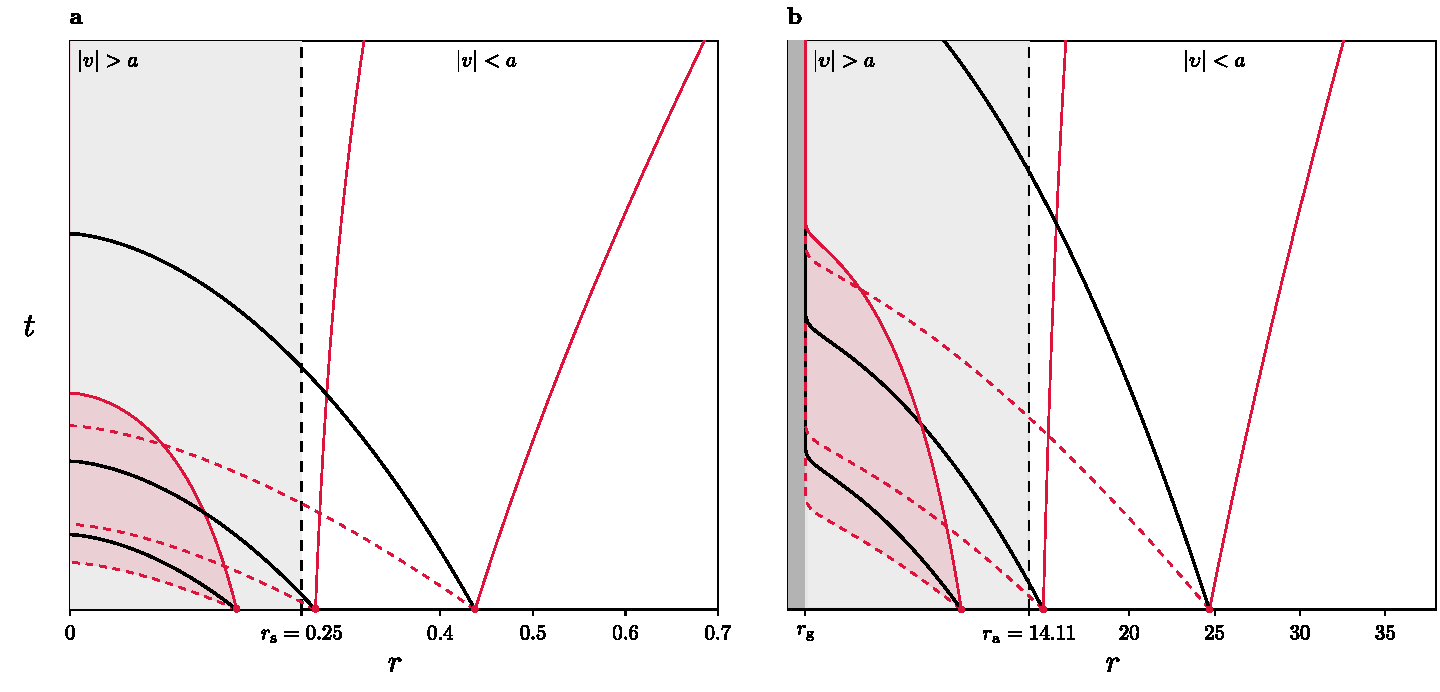
\includegraphics[width=\linewidth]{causal_structure.pdf}
\caption{Причинная структура двух течений в плоскости $(r,t)$; время растёт вверх, масштаб по нему в каждой панели свой. (a)~Ньютоновское течение Бонди в абсолютном времени ($r_{\mathrm{s}}=0.25\,r_{\mathrm{B}}$). (b)~Течение Мишеля в координатах Шварцшильда при $a_{\infty}=0.1$ ($r_{\mathrm{a}}=14.11\,r_{\mathrm{g}}$) -- тот же фон, что и в панели~(b) рис.~\ref{fig:mach_topology}. Оба течения взяты при $\gamma=4/3$: значение $5/3$ здесь непригодно, поскольку звуковая точка Бонди при нём уходит в центр. Малиновые точки -- события испускания: в панели~(a) они лежат при $r=0.18$, $0.27$ и $0.44\,r_{\mathrm{B}}$, в панели~(b) -- при $r=10.2$, $15.0$ и $24.7\,r_{\mathrm{g}}$. В обоих течениях это одни и те же доли радиуса акустического горизонта, $0.72$, $1.06$ и $1.75$, а сами радиусы различаются лишь потому, что различаются горизонты: $r_{\mathrm{s}}=0.25\,r_{\mathrm{B}}$ у Бонди против $r_{\mathrm{a}}=14.11\,r_{\mathrm{g}}$ у Мишеля. Из каждого события выпущены обе звуковые характеристики: сплошная малиновая -- исходящая, штриховая -- входящая; чёрные кривые -- мировые линии жидкости, единственная характеристика инвариантов $\delta\omega_{\mu\nu}$ и $\delta S$. Скорости характеристик даны уравнением~\eqref{eq:acoustic_surface_gravity} для течения Мишеля и простой суммой $v_{\pm}=v\pm a$ для течения Бонди. Серая полоса -- сверхзвуковая оболочка, вертикальный пунктир -- акустический горизонт, где $v_{+}=0$: внутри оболочки обе звуковые ветви направлены внутрь, и область влияния события (заливка) горизонт не покидает, а снаружи исходящая ветвь уходит наружу, но у горизонта замирает линейно по расстоянию до него. Это замирание одинаково в обоих течениях и даёт то самое логарифмическое растяжение с поверхностной гравитацией $\kappa$. Различаются внутренние концы. У Бонди за акустическим горизонтом стоит сама точечная масса, и звуковые лучи вместе с мировыми линиями доходят до $r=0$ за конечное время. У Мишеля же внутренним концом служит гравитационный горизонт (тёмная полоса): загиб кривых в вертикаль при $r\rightarrow r_{\mathrm{g}}$ -- координатная особенность Шварцшильда, а не физическое замирание, но именно из-за неё координатное время падения бесконечно. Замена точечной массы чёрной дырой убирает внутреннюю границу вместе с ней.}
\label{fig:causal_structure}
\end{figure}

\subsection{Линеаризованные уравнения гидродинамики}
\label{sec:linearized_system}

Динамика идеальной релятивистской жидкости определяется сохранением частиц, уравнением Эйлера в форме Лихнеровича -- Крокко и переносом энтропии,
\begin{equation}
    \nabla_{\mu}(nu^{\mu})=0,
    \label{eq:continuity}
\end{equation}
\begin{equation}
    u^{\mu}\omega_{\mu\nu}=T\,\partial_{\nu}S,
    \label{eq:euler_crocco}
\end{equation}
\begin{equation}
    \omega_{\mu\nu}
    \equiv
    \partial_{\mu}(hu_{\nu})-\partial_{\nu}(hu_{\mu}),
    \label{eq:vorticity_definition}
\end{equation}
\begin{equation}
    u^{\mu}\partial_{\mu}S=0,
    \label{eq:entropy_advection}
\end{equation}
где $T$ -- температура, а $\omega_{\mu\nu}$ -- завихрённость обобщённого импульса $hu_{\mu}$. Мы линеаризуем эту систему на гомэнтропическом безвихревом фоне Мишеля, для которого $\partial_{\mu}S=0$ и $\omega_{\mu\nu}=0$, полагая
\begin{equation}
    n\rightarrow n+\delta n,\quad
    h\rightarrow h+\delta h,\quad
    u^{\mu}\rightarrow u^{\mu}+\delta u^{\mu},\quad
    S\rightarrow S+\delta S,
    \label{eq:perturbation_expansion}
\end{equation}
и удерживая только члены первого порядка. Нормировка~\eqref{eq:four_velocity_normalization} сразу требует ортогональности возмущения скорости потоку,
\begin{equation}
    u_{\mu}\delta u^{\mu}=0.
    \label{eq:velocity_orthogonality}
\end{equation}

Термодинамические возмущения не все независимы. Поскольку течение теперь несёт энтропию, вариацию плотности берём по двум направлениям -- энтальпийному и энтропийному,
\begin{equation}
    \delta n
    =
    \frac{n}{ha^{2}}\,\delta h
    +\left(\frac{\partial n}{\partial S}\right)_{h}\delta S
    =
    n\left(\frac{\delta h}{ha^{2}}+\chi\,\delta S\right),
    \label{eq:thermodynamic_perturbation}
\end{equation}
где введена энтропийная восприимчивость
\begin{equation}
    \chi
    \equiv
    \frac{1}{n}\left(\frac{\partial n}{\partial S}\right)_{h}.
    \label{eq:chi_definition}
\end{equation}
При естественной политропной нормировке энтропии $S=\ln K$ (с соответственно перенормированной сопряжённой температурой) эта восприимчивость постоянна, $\chi=-(\gamma-1)^{-1}$, а привычное адиабатическое соотношение $\delta n=n\,\delta h/(ha^{2})$ восстанавливается лишь при $\delta S=0$. Подставляя $\delta n$ в уравнение непрерывности~\eqref{eq:continuity}, получаем его линеаризованную форму,
\begin{equation}
    \nabla_{\mu}
    \left\{
        n\left[
            \delta u^{\mu}
            +u^{\mu}\left(
                \frac{\delta h}{ha^{2}}+\chi\,\delta S
            \right)
        \right]
    \right\}
    =0.
    \label{eq:linearized_continuity}
\end{equation}

Уравнение Эйлера удобнее всего линеаризовать через возмущение импульса-одной-формы и его завихрённость,
\begin{equation}
    w_{\mu}
    \equiv
    \delta(hu_{\mu})
    =
    h\,\delta u_{\mu}+u_{\mu}\delta h,
    \qquad
    \delta\omega_{\mu\nu}
    =
    \partial_{\mu}w_{\nu}-\partial_{\nu}w_{\mu},
    \label{eq:perturbed_momentum}
\end{equation}
в терминах которых уравнения Крокко и энтропии для фонового течения Мишеля сводятся к
\begin{equation}
    u^{\mu}\delta\omega_{\mu\nu}
    =T\,\partial_{\nu}\delta S,
    \label{eq:linearized_euler}
\end{equation}
\begin{equation}
    u^{\mu}\partial_{\mu}\delta S=0,
    \label{eq:linearized_entropy}
\end{equation}
Вместе с термодинамическим соотношением~\eqref{eq:thermodynamic_perturbation} уравнения \eqref{eq:linearized_continuity}, \eqref{eq:linearized_euler} и \eqref{eq:linearized_entropy} образуют полную систему первого порядка, используемую в остальной части статьи.

Стационарность и сферическая симметрия позволяют разделить переменные: любое скалярное возмущение раскладывается как
\begin{equation}
    \delta Q(t,r,\theta,\phi)
    =
    \sum_{\ell m}
    \widetilde{Q}_{\ell m}(r)
    Y_{\ell m}(\theta,\phi)e^{-i\omega t}.
    \label{eq:harmonic_decomposition}
\end{equation}
Временная и радиальная компоненты $w_{\mu}$ раскладываются по скалярным сферическим гармоникам, тогда как угловые компоненты $w_{A}$ -- по соответствующим векторным сферическим гармоникам, так что секторы $(\ell,m,\omega)$ в линейном порядке развязываются. Во всём анализе пространственной устойчивости $\omega$ считается вещественной, и вопрос состоит в том, остаётся ли возмущение заданной частоты ограниченным при переносе к чёрной дыре.

То же разложение делит возмущение скорости, измеренное локально покоящимся наблюдателем, на радиальную, полярную и тороидальную части:
\begin{equation}
    \delta\boldsymbol{v}
    =
    \Bigl[
        \delta v_{\mathrm{rad}}(r)\,Y_{\ell m}\,\boldsymbol{e}_{r}
        +
        \delta v_{\mathrm{pol}}(r)\,
        r\boldsymbol{\nabla}_{\!\mathrm{T}}Y_{\ell m}
        +
        \delta v_{\mathrm{tor}}(r)\,
        \boldsymbol{e}_{r}\times r\boldsymbol{\nabla}_{\!\mathrm{T}}Y_{\ell m}
    \Bigr]e^{-i\omega t},
    \label{eq:velocity_amplitudes}
\end{equation}
где $\boldsymbol{\nabla}_{\!\mathrm{T}}
=r^{-1}\boldsymbol{e}_{\theta}\partial_{\theta}
+(r\sin\theta)^{-1}\boldsymbol{e}_{\phi}\partial_{\phi}$ -- тангенциальный градиент на сфере. Полярная часть градиентна и потому сопровождается сжатием газа, тогда как тороидальная бездивергентна и возмущения плотности не создаёт; при $\ell=0$ обе угловые части исчезают, и остаётся одна радиальная амплитуда. В ньютоновском пределе $\delta\boldsymbol{v}$ -- обычное возмущение трёхмерной скорости, а на фоне Мишеля -- пространственные компоненты $\delta u_{\mu}$ в локально ортонормированном базисе статического наблюдателя; поскольку вся рассматриваемая область лежит вне гравитационного горизонта, $r\geq r_{\mathrm{a}}>r_{\mathrm{g}}$, эти два набора компонент связаны гладкими конечными множителями и показатели степеней у амплитуд от выбора базиса не зависят. Всюду ниже амплитуды измеряются относительно фона: плотность -- в виде $\delta n/n$ (или $\delta\rho/\rho$ в ньютоновском пределе), скорость -- в единицах местной скорости звука $a$.

Зафиксировав это гармоническое представление, можно перейти к разложению возмущения на акустическую, вихревую и энтропийную составляющие.

\subsection{Разложение на акустические, вихревые и энтропийные моды}
\label{sec:mode_decomposition}

Завихрённость отделяет потенциальные возмущения от вихревых. Соответственно, возмущение обобщённого импульса разбиваем на потенциальную часть и вихревой остаток,
\begin{equation}
    w_{\mu}
    =
    \partial_{\mu}\delta\varphi+w_{\mu}^{\perp},
    \qquad
    \delta\omega_{\mu\nu}
    =
    \partial_{\mu}w_{\nu}^{\perp}
    -
    \partial_{\nu}w_{\mu}^{\perp}.
    \label{eq:helmholtz_decomposition}
\end{equation}
так что потенциальный отклик содержится в $\delta\varphi$, а вся завихрённость -- в $w_{\mu}^{\perp}$. Три семейства мод тогда классифицируются следующим образом:
\begin{center}
    \small
    \setlength{\tabcolsep}{4pt}
    \renewcommand{\arraystretch}{1.1}
    \begin{tabularx}{\textwidth}{
        >{\raggedright\arraybackslash}p{3.0cm}
        >{\centering\arraybackslash}p{1.2cm}
        >{\centering\arraybackslash}p{3.8cm}
        >{\raggedright\arraybackslash}X}
        \toprule
        Сектор & $\delta S$ & $\delta\omega_{\mu\nu}$ & Динамика \\
        \midrule
        Акустический & $0$ & $0$ & распространение на акустическом конусе \\
        Вихревой & $0$ & $\neq0$ & адвекция с жидкостью \\
        Энтропийный & $\neq0$ & в общем случае с источником & адвекция и вынужденный отклик \\
        \bottomrule
    \end{tabularx}
\end{center}
Это релятивистский аналог классификации акустических, вихревых и энтропийных возмущений, известной из теории сжимаемых течений~\cite{KovasznayLSG_TurbulenceInSupersonicFlow_1953}.

Для акустических возмущений $\delta\omega_{\mu\nu}=0$, поэтому локально $w_{\mu}=\partial_{\mu}\delta\varphi$. С другой стороны, $w_{\mu}=h\,\delta u_{\mu}+u_{\mu}\delta h$. Сворачивая с $u^{\mu}$ и используя~\eqref{eq:velocity_orthogonality}, находим
\begin{equation}
    \delta h=-u^{\mu}\partial_{\mu}\delta\varphi.
    \label{eq:acoustic_enthalpy}
\end{equation}
Тогда ортогональная к потоку часть даёт
\begin{equation}
    h\,\delta u_{\mu}
    =
    \left(\delta_{\mu}^{\nu}+u_{\mu}u^{\nu}\right)
    \partial_{\nu}\delta\varphi.
    \label{eq:acoustic_fields}
\end{equation}
Подстановка этих выражений в изоэнтропическую форму~\eqref{eq:linearized_continuity} сводит систему к однородному волновому уравнению на $\delta\varphi$, которое анализируется в разд.~\ref{sec:acoustic}.

Если $\delta S=0$, но $\delta\omega_{\mu\nu}\neq0$, то уравнение~\eqref{eq:linearized_euler} сводится к
\begin{equation}
    u^{\mu}\delta\omega_{\mu\nu}=0.
    \label{eq:vortex_frozen}
\end{equation}
Тем самым в изоэнтропическом секторе ($\delta S=0$) бароклинное порождение завихрённости отсутствует, а существующее вихревое возмущение остаётся вмороженным в фоновое течение. Тем не менее, подстановка $w_{\mu}=\partial_{\mu}\delta\varphi+w_{\mu}^{\perp}$ в уравнение непрерывности~\eqref{eq:linearized_continuity} показывает, что $w_{\mu}^{\perp}$ служит источником акустического потенциала; соответствующее вынужденное волновое уравнение выводится в разд.~\ref{sec:vortical}.

Если $\delta S\neq0$, энтропийное возмущение адвектируется вдоль линий тока
\begin{equation}
    u^{\mu}\partial_{\mu}\delta S=0,
    \label{eq:entropy_mode_advection}
\end{equation}
а его градиент служит бароклинным источником завихрённости
\begin{equation}
    u^{\mu}\delta\omega_{\mu\nu}
    =
    T\,\partial_{\nu}\delta S.
    \label{eq:entropy_vorticity_source}
\end{equation}
Возникшая завихрённость, в свою очередь, может возбуждать звук через уравнение непрерывности. Соответствующая связь с энтропийной модой выводится в разд.~\ref{sec:entropy}.

\section{Акустические моды и пространственная устойчивость}
\label{sec:acoustic}

\subsection{Волновое уравнение и приведение к шрёдингеровой форме}
\label{sec:acoustic_wave_equation}

Для свободного акустического сектора уравнения~\eqref{eq:acoustic_enthalpy} и~\eqref{eq:acoustic_fields} сводят линеаризованную систему к
\begin{equation}
    \partial_{\mu}
    \left(
        \sqrt{-g}\,\Omega^{2}\eta^{\mu\nu}
        \partial_{\nu}\delta\varphi
    \right)=0,
    \qquad
    \Omega^{2}\equiv\frac{n}{h},
    \label{eq:acoustic_wave_equation}
\end{equation}
где $\sqrt{-g}=r^{2}\sin\theta$ для фона Шварцшильда. Чтобы явно выделить лучевой предел, введём эйкональный анзац $\delta\varphi=A\exp(i\omega\mathcal{S})$ и волновой ковектор $k_{\mu}=\partial_{\mu}\mathcal{S}$. В главном порядке по $\omega$ уравнение~\eqref{eq:acoustic_wave_equation} даёт
\begin{equation}
    \eta^{\mu\nu}k_{\mu}k_{\nu}=0.
    \label{eq:acoustic_eikonal_relation}
\end{equation}
Конформный множитель $\Omega^{2}$ выпадает из этого условия и потому не влияет на звуковые лучи. Однако он остаётся под производной в уравнении~\eqref{eq:acoustic_wave_equation}, поэтому амплитуды конечной частоты зависят от профилей плотности и энтальпии даже тогда, когда лучевые траектории от них не зависят.

Для одной гармоники
\begin{equation}
    \delta\varphi
    =
    \operatorname{Re}
    \left[
        \delta\widetilde{\varphi}(r)Y_{\ell m}(\theta,\phi)e^{-i\omega t}
    \right],
    \label{eq:acoustic_separation}
\end{equation}
волновое уравнение принимает вид
\begin{equation}
    A\delta\widetilde{\varphi}''
    +B\delta\widetilde{\varphi}'
    +C\delta\widetilde{\varphi}=0,
    \label{eq:radial_master_equation}
\end{equation}
где
\begin{equation}
    A=P\eta^{rr},
    \quad
    B=(P\eta^{rr})'-2i\omega P\eta^{rt},
    \quad
    C=-\omega^{2}P\eta^{tt}
       -i\omega(P\eta^{rt})'
       -\Omega^{2}\ell(\ell+1),
    \quad
    P\equiv r^{2}\Omega^{2}.
    \label{eq:radial_coefficients}
\end{equation}
Штрихи обозначают $\mathrm{d}/\mathrm{d}r$. Мнимые члены возникают из недиагональных компонент ядра акустической метрики~$\eta^{\mu\nu}$ вследствие адвекции фоновым течением, которая приводит к смешиванию временных и радиальных производных акустического возмущения.

Эти мнимые члены можно устранить, выделив адвективную фазу:
\begin{equation}
    \delta\widetilde{\varphi}(r)=
    \exp\left(i\omega\int^{r}\frac{\eta^{rt}}{\eta^{rr}}\,\mathrm{d}r'\right)\varrho(r).
    \label{eq:phase_transformation}
\end{equation}
Используя точное тождество
\begin{equation}
    \eta^{tt}\eta^{rr}-(\eta^{rt})^{2}=-a^{-2},
    \label{eq:core_determinant}
\end{equation}
получаем из уравнения~\eqref{eq:radial_master_equation} вещественное самосопряжённое уравнение
\begin{equation}
    \left(P\eta^{rr}\varrho'\right)'
    +
    \left[
        \omega^{2}\frac{P}{a^{2}\eta^{rr}}
        -\Omega^{2}\ell(\ell+1)
    \right]\varrho=0.
    \label{eq:sturm_liouville}
\end{equation}
Во внешней области, где $\eta^{rr}>0$, уравнение~\eqref{eq:sturm_liouville} приводится к шрёдингеровой форме введением волновой акустической черепашьей координаты $r_{*}$ и мастер-переменной $X$, представляющей собой перенормированную радиальную функцию $\varrho$:
\begin{equation}
    \frac{\mathrm{d}r_{*}}{\mathrm{d}r}
    =
    \frac{1}{a\eta^{rr}},
    \qquad
    X\equiv\sqrt{W}\,\varrho,
    \qquad
    W\equiv\frac{r^{2}\Omega^{2}}{a}.
    \label{eq:tortoise_rescaling}
\end{equation}
Определённая таким образом координата $r_{*}$ имеет ту же поверхностную гравитацию, что и лучевая черепашья координата $\mathrm{d}r=v_{+}\,\mathrm{d}r_{*}^{\mathrm{(ray)}}$, введённая в~\cite{SemyannikovAV_AcousticGeometryAndSoundRayDynamics_2026}, хотя глобально эти координаты различаются. Ниже входящие и исходящие волны, а следовательно, и амплитуды рассеяния определяются относительно волновой координаты $r_{*}$. В новых переменных радиальное уравнение принимает шрёдингерову форму
\begin{equation}
    \frac{\mathrm{d}^{2}X}{\mathrm{d}r_{*}^{2}}
    +
    \left[\omega^{2}-V_{\mathrm{eff}}(r)\right]X=0,
    \label{eq:schrodinger_equation}
\end{equation}
где
\begin{equation}
    V_{\mathrm{eff}}
    =
    \frac{\ell(\ell+1)}{r^{2}}a^{2}\eta^{rr}
    +
    \frac{1}{\sqrt{W}}
    \frac{\mathrm{d}^{2}\sqrt{W}}{\mathrm{d}r_{*}^{2}}.
    \label{eq:effective_potential}
\end{equation}
Первый член является обобщённым центробежным барьером: он пропорционален $\ell(\ell+1)$ и совпадает с лучевым барьером захвата в эйкональном пределе большого углового момента. Второй член порождён радиальными изменениями скорости звука, плотности и энтальпии через весовой множитель $W$; он управляет амплитудами конечной частоты и отсутствует в геометрической оптике.

Прежде чем переходить к фону Мишеля, убедимся, что редукция~\eqref{eq:schrodinger_equation}--\eqref{eq:effective_potential} воспроизводит вакуумный предел. Если формально отключить отклик жидкости, положив $a\rightarrow1$, $\upsilon\rightarrow0$ и $\Omega\rightarrow\mathrm{const}$, то акустическая геометрия вырождается в геометрию Шварцшильда: $\eta^{rr}\rightarrow f$, $\mathrm{d}r_{*}/\mathrm{d}r\rightarrow f^{-1}$ и $W\propto r^{2}$. Эффективный потенциал при этом принимает вид
\begin{equation}
    V_{\mathrm{eff}}
    \longrightarrow
    f\left[
        \frac{\ell(\ell+1)}{r^{2}}+\frac{1}{r^{3}}
    \right],
    \label{eq:scalar_schwarzschild_potential}
\end{equation}
то есть совпадает с безразмерным потенциалом безмассового скалярного поля. Тем самым воспроизводятся и стандартная черепашья координата Шварцшильда, и вклад перенормировки на $W$, дающий член $\sim f/r^{3}$ в скалярном потенциале.

Полученное уравнение и определяет акустический сектор течения Мишеля. Область его решений ограничена изнутри акустическим горизонтом, а не центром притяжения, поэтому сначала выясним, как ведут себя решения на её концах.

\subsection{Граничные асимптотики и индициальный анализ}
\label{sec:boundary_asymptotics}

На пространственной бесконечности течение Мишеля выходит на однородное состояние: радиальная скорость обращается в нуль, а скорость звука и конформный множитель стремятся к своим асимптотическим значениям $a_{\infty}$ и $\Omega_{\infty}$. Черепашья координата тогда становится пропорциональной радиусу, $r_{*}\sim r/a_{\infty}$, а эффективный потенциал убывает до нуля. Поэтому шрёдингерово уравнение~\eqref{eq:schrodinger_equation} допускает обычную суперпозицию входящей и исходящей волн,
\begin{equation}
    X\sim
    A_{\mathrm{in}}e^{-i\omega r_{*}}
    +
    A_{\mathrm{out}}e^{i\omega r_{*}},
    \qquad r_{*}\rightarrow+\infty.
    \label{eq:infinity_asymptotics}
\end{equation}

Внутренней границей внешней задачи служит акустический горизонт $r=r_{\mathrm{a}}$. Введём локальную координату $x=r-r_{\mathrm{a}}$. Для невырожденного трансзвукового решения радиальная компонента акустического ядра имеет простой нуль,
\begin{equation}
    \eta^{rr}=q_{1}x+\mathcal{O}(x^{2}),
    \qquad
    q_{1}\equiv
    \left.\frac{\mathrm{d}\eta^{rr}}{\mathrm{d}r}\right|_{r_{\mathrm{a}}}
    >0,
    \label{eq:horizon_expansion}
\end{equation}
поэтому черепашья координата~\eqref{eq:tortoise_rescaling} логарифмически уходит на минус бесконечность:
\begin{equation}
    r_{*}
    =
    \frac{1}{a_{\mathrm{a}}q_{1}}\ln x+\mathcal{O}(1)
    \longrightarrow-\infty.
    \label{eq:tortoise_horizon}
\end{equation}
Вблизи горизонта эффективный потенциал стремится к нулю, поэтому уравнение~\eqref{eq:schrodinger_equation} локально описывает свободные бегущие волны. Однако акустический горизонт является односторонней границей: при выбранной временной зависимости $e^{-i\omega t}$ звуковая волна не может выйти из сверхзвуковой области во внешнюю. Поэтому физическое решение рассеяния содержит только ветвь, направленную вдоль потока,
\begin{equation}
    X\sim A_{\mathrm{tr}}e^{-i\omega r_{*}},
    \qquad r_{*}\rightarrow-\infty.
    \label{eq:horizon_boundary_condition}
\end{equation}
Здесь $A_{\mathrm{tr}}$ обозначает амплитуду волны, прошедшей через акустический горизонт.

Локальное поведение исходной радиальной амплитуды $\delta\widetilde{\varphi}$ можно получить непосредственно из уравнения~\eqref{eq:radial_master_equation}. Простой нуль $\eta^{rr}$ приводит к линейному обращению в нуль коэффициента при старшей производной,
\begin{equation}
    A=A_{1}x+\mathcal{O}(x^{2}),
    \qquad
    A_{1}=r_{\mathrm{a}}^{2}\Omega_{\mathrm{a}}^{2}q_{1}.
\end{equation}
Подставляя анзац Фробениуса $\delta\widetilde{\varphi}\sim x^{\sigma}$ и сохраняя ведущие по $x$ члены, получаем индициальное уравнение и его корни:
\begin{equation}
    \sigma
    \left(
        \sigma-\frac{2i\omega\eta^{rt}_{\mathrm{a}}}{q_{1}}
    \right)=0,
    \qquad
    \sigma_{1}=0,
    \qquad
    \sigma_{2}
    =
    \frac{2i\omega\eta^{rt}_{\mathrm{a}}}{q_{1}}.
    \label{eq:horizon_indicial}
\end{equation}
Для входящего течения Мишеля $\eta^{rt}_{\mathrm{a}}=a_{\mathrm{a}}^{-1}>0$, поэтому второй показатель является чисто мнимым: соответствующая ветвь осциллирует по $\ln x$, но не растёт по модулю.

Логарифмическое растяжение исходящих звуковых характеристик вблизи горизонта определяется акустической поверхностной гравитацией $\kappa$. Подробный вывод этой связи для звуковых лучей течения Мишеля приведён в~\cite{SemyannikovAV_AcousticGeometryAndSoundRayDynamics_2026}. Здесь, обозначая через $v_{+}=(\mathrm{d}r/\mathrm{d}t)_{+}$ координатную скорость исходящего звукового луча, определим $\kappa$ как
\begin{equation}
    \kappa
    \equiv
    \frac{1}{2}
    \left.
    \frac{\mathrm{d}v_{+}}{\mathrm{d}r}
    \right|_{r=r_{\mathrm{a}}}.
    \label{eq:acoustic_surface_gravity}
\end{equation}
Поскольку $v_{+}$ линейно обращается в нуль на горизонте,
\begin{equation}
    v_{+}=2\kappa x+\mathcal{O}(x^{2}),
    \qquad
    r_{*}^{\mathrm{(ray)}}
    =
    \int\frac{\mathrm{d}r}{v_{+}}
    =
    \frac{1}{2\kappa}\ln x+\mathcal{O}(1).
\end{equation}
Лучевая и волновая черепашьи координаты различаются вдали от горизонта, но имеют один и тот же логарифмический коэффициент. Сравнение с уравнением~\eqref{eq:tortoise_horizon} поэтому даёт
\begin{equation}
    2\kappa=a_{\mathrm{a}}q_{1},
    \qquad
    \sigma_{2}=\frac{i\omega}{\kappa}.
    \label{eq:horizon_exponent_surface_gravity}
\end{equation}
С учётом адвективной фазы~\eqref{eq:phase_transformation} постоянная ветвь $\sigma_{1}=0$ соответствует входящему мастер-решению $X\sim e^{-i\omega r_{*}}$, тогда как осциллирующая ветвь $\sigma_{2}$ соответствует исходящему решению. В терминах исходной радиальной амплитуды две локальные ветви имеют вид
\begin{equation}
    \delta\widetilde{\varphi}_{\mathrm{Michel}}
    \sim
    C_{\mathrm{in}}
    +
    C_{\mathrm{out}}\,x^{i\omega/\kappa},
    \qquad
    r \rightarrow r_{\mathrm{a}}.
    \label{eq:michel_local_branches}
\end{equation}
Здесь $C_{\mathrm{in}}$ и $C_{\mathrm{out}}$ -- произвольные комплексные амплитуды входящей и исходящей ветвей соответственно. Поскольку $\omega$ вещественна, $\lvert x^{i\omega/\kappa}\rvert=1$, поэтому при $r\rightarrow r_{\mathrm{a}}$ ни одна из ветвей не растёт по модулю.

Критерий устойчивости, однако, относится не к самому потенциалу, а к физическим полям, восстанавливаемым из его производных. Фоновые профили и коэффициенты уравнения~\eqref{eq:radial_master_equation} гладки при $r=r_{\mathrm{a}}$, а входящая ветвь аналитична, $\delta\widetilde{\varphi}=C_{\mathrm{in}}\left[1+\mathcal{O}(x)\right]$, поэтому уравнения~\eqref{eq:acoustic_enthalpy} и~\eqref{eq:acoustic_fields} дают для неё конечные пределы всех амплитуд~\eqref{eq:velocity_amplitudes}:
\begin{equation}
    C_{\mathrm{out}}=0:
    \quad
    \frac{\delta n}{n},\
    \frac{\delta v_{\mathrm{rad}}}{a},\
    \frac{\delta v_{\mathrm{pol}}}{a}
    \sim x^{0};
    \qquad
    C_{\mathrm{out}}\neq0:
    \quad
    \frac{\delta n}{n},\
    \frac{\delta v_{\mathrm{rad}}}{a}
    \sim x^{-1},
    \quad
    \frac{\delta v_{\mathrm{pol}}}{a}
    \sim x^{0}.
    \label{eq:michel_acoustic_horizon_asymptotics}
\end{equation}
Тороидальная амплитуда в этом секторе отсутствует: течение потенциально, $\delta\boldsymbol{v}=\boldsymbol{\nabla}\delta\varphi$. Показатели не зависят от $\ell$, поскольку угловой член в уравнении~\eqref{eq:effective_potential} пропорционален $\eta^{rr}$ и на горизонте обращается в нуль. Расходимость второй группы отвечает исходящей ветви, у которой $\delta\widetilde{\varphi}'\sim x^{i\omega/\kappa-1}$; это обычная особенность исходящих решений на горизонте, и физическое граничное условие~\eqref{eq:horizon_boundary_condition} её исключает.

Итак, во внешней задаче Мишеля все относительные амплитуды выходят у горизонта на конечные значения. Установленная регулярность относится именно к области $r\geq r_{\mathrm{a}}$: продолжение решения через сверхзвуковую оболочку к гравитационному горизонту требует отдельного анализа в проникающих координатах и здесь не рассматривается. Чтобы понять, насколько этот результат отличается от ньютоновского, вернёмся к пределу Бонди.

\subsection{Ньютоновский предел и асимптотики Бонди}
\label{sec:newtonian_bondi_acoustic}

Вторую, независимую проверку редукции даёт ньютоновский предел, в котором
\begin{equation}
    f\rightarrow1,\qquad
    h\rightarrow1,\qquad
    a\ll1,\qquad
    |\upsilon|\ll1,
    \qquad
    \frac{|\upsilon|}{a}=\mathcal{O}(1),
    \qquad
    \Omega^{2}\rightarrow\rho,
    \label{eq:newtonian_limit}
\end{equation}
а временно-радиальный блок волнового оператора сводится к акустическому ядру Унру--Виссера~\cite{UnruhWG_ExperimentalBlackHoleEvaporation_1981,VisserM_AcousticBlackHolesHorizonsErgospheresAndHawkingRadiation_1998}:
\begin{equation}
    \Omega^{2}\eta^{AB}
    \longrightarrow
    \frac{\rho}{a^{2}}
    \begin{pmatrix}
        -1 & -\upsilon\\
        -\upsilon & a^{2}-\upsilon^{2}
    \end{pmatrix},
    \qquad A,B\in\{t,r\}.
    \label{eq:newtonian_acoustic_core}
\end{equation}
После разделения переменных уравнение~\eqref{eq:radial_master_equation} переходит в радиальное волновое уравнение задачи Бонди, полученное в работе~\cite{KovalenkoIG_EreminMA_SpatialInstabilityOfSphericalAccretion_1998},
\begin{equation}
    (a^{2}-\upsilon^{2})\delta\widetilde{\varphi}''
    +
    \left[
        2i\omega\upsilon
        -(a^{2}+\upsilon^{2})\frac{\upsilon'}{\upsilon}
        +2\upsilon^{2}\frac{a'}{a}
    \right]\delta\widetilde{\varphi}'
    +
    \left[
        \omega^{2}
        -2i\omega\upsilon\frac{a'}{a}
        -\ell(\ell+1)\frac{a^{2}}{r^{2}}
    \right]\delta\widetilde{\varphi}=0.
    \label{eq:kovalenko_eremin_limit}
\end{equation}
Такое совпадение подтверждает правильность волнового оператора и одновременно задаёт точку отсчёта для сравнения.

Область этой задачи доходит до самой точечной массы, и её внутренним концом служит регулярная особая точка $r=0$; насколько это меняет постановку, видно уже из сравнения самих фоновых течений на рис.~\ref{fig:mach_topology}, где аккреционная ветвь Бонди продолжается до сколь угодно малых радиусов, а у Мишеля обрывается на горизонте при конечном числе Маха. У критического течения Бонди газ подходит к внутреннему концу в режиме свободного падения,
\begin{equation}
    |\upsilon|\sim r^{-1/2},
    \qquad
    \rho\sim r^{-3/2},
    \qquad
    a\sim r^{-3(\gamma-1)/4},
    \label{eq:bondi_freefall_asymptotics}
\end{equation}
и индициальный анализ уравнения~\eqref{eq:kovalenko_eremin_limit} в этой точке даёт две локальные ветви~\cite{KovalenkoIG_EreminMA_SpatialInstabilityOfSphericalAccretion_1998}
\begin{equation}
    \delta\widetilde{\varphi}_{\mathrm{Bondi}}
    \sim
    C_{\mathrm{reg}}+C_{\mathrm{pow}}\,r^{\sigma},
    \qquad
    \sigma=\frac{6-3\gamma}{2},
    \qquad
    r\rightarrow0,
    \label{eq:bondi_local_branches}
\end{equation}
где $C_{\mathrm{reg}}$ и $C_{\mathrm{pow}}$ -- амплитуды постоянной (регулярной) и степенной ветвей. В отличие от чисто мнимого показателя~\eqref{eq:horizon_exponent_surface_gravity}, оба показателя здесь вещественны, поэтому решения меняются по степенному закону, а не осциллируют по логарифму расстояния до внутренней границы. Сам потенциал при этом остаётся ограниченным: постоянная ветвь стремится к константе, а степенная -- к нулю при $\sigma>0$.

\begin{figure}[!tb]
\centering
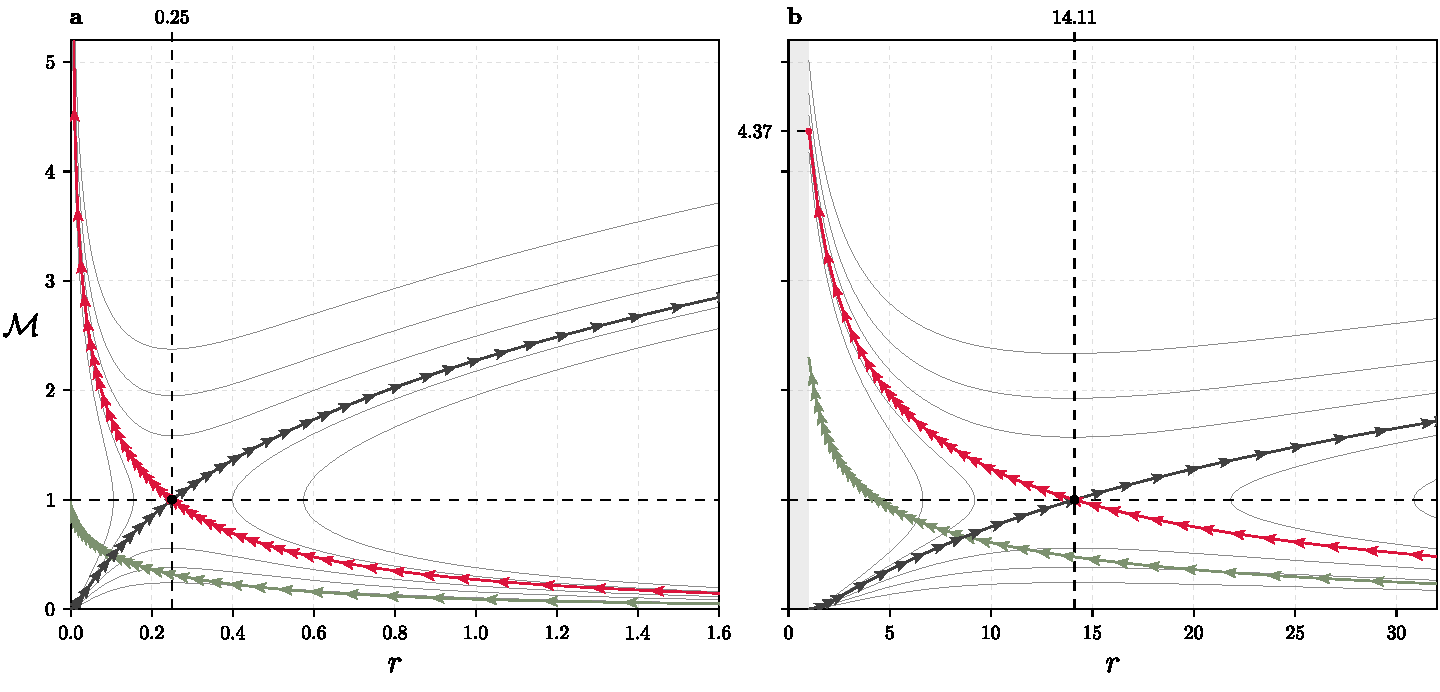
\includegraphics[width=\linewidth]{mach_topology.pdf}
\caption{Топология стационарных решений в плоскости $(r,\mathcal{M})$ в линейных осях: (a)~течение Бонди, число Маха $\mathcal{M}=v/a$, радиус в единицах радиуса Бонди $r_{\mathrm{B}}=GM/a_{\infty}^{2}$; (b)~течение Мишеля при $a_{\infty}=0.1$, физическое число Маха $\mathcal{M}=V/a$, где $V=|\upsilon|/\sqrt{f+\upsilon^{2}}$ -- скорость, измеряемая локально покоящимся наблюдателем, радиус в единицах гравитационного радиуса $r_{\mathrm{g}}$. При фиксированном интеграле Бернулли каждое решение есть линия уровня потока $\mathcal{J}$ ($r^{2}\rho v$ у Бонди, $r^{2}n\upsilon$ у Мишеля), поэтому всё семейство решений -- набор линий уровня одной функции $\mathcal{J}(r,\mathcal{M})$; тонкие серые кривые отвечают некритическим значениям $\mathcal{J}\neq\mathcal{J}_{\mathrm{c}}$. Критическому потоку при $\gamma=4/3$ отвечает пара выделенных кривых, пересекающихся в звуковой точке: красная -- аккреционная ветвь $\upsilon<0$, тёмная -- ветвь ветра $\upsilon>0$; стрелки на них указывают направление течения. Зелёная кривая -- критическая аккреционная ветвь при $\gamma=5/3$, второе используемое в статье значение. Горизонтальный пунктир -- уровень $\mathcal{M}=1$, вертикальный -- звуковая точка, её радиус подписан сверху ($0.25\,r_{\mathrm{B}}$ и $14.11\,r_{\mathrm{g}}$). Звуковая точка -- седло семейства, а трансзвуковое решение -- его сепаратриса: серые линии уровня либо остаются всюду до- или сверхзвуковыми, достигая экстремума числа Маха в звуковой точке, либо поворачивают на $\mathcal{M}=1$, не доходя до неё. Внутренние границы двух задач устроены по-разному, и в линейных осях это различие видно сразу. У Бонди внутренний конец лежит в самом центре, и там семейство расходится: дозвуковые ветви приходят в начало координат как $\mathcal{M}\propto r^{(5-3\gamma)/[2(\gamma-1)]}$, а сверхзвуковые прижимаются к оси ординат и уходят за верхний край рамки как $\mathcal{M}\propto r^{(3\gamma-5)/4}$. Оба показателя пропорциональны $5-3\gamma$ и обращаются в нуль при $\gamma=5/3$: зелёная кривая в панели~(a) дозвуковая на всех конечных радиусах и подходит к $\mathcal{M}=1$ лишь в самой точке $r=0$, куда стягивается звуковая точка $r_{\mathrm{s}}=(5-3\gamma)r_{\mathrm{B}}/4$, так что X-образной особенности на конечном радиусе не остаётся вовсе. У Мишеля, наоборот, область обрывается на гравитационном горизонте (серая полоса $r<r_{\mathrm{g}}$), и сверхзвуковые ветви приходят туда с конечными числами Маха: у красной ветви это $\mathcal{M}=4.37$ (отметка на оси ординат). Смена показателя адиабаты здесь ничего не ломает: зелёная ветвь при $\gamma=5/3$ лишь сдвинута внутрь вместе с акустическим горизонтом ($r_{\mathrm{a}}=4.38\,r_{\mathrm{g}}$ вместо $14.11\,r_{\mathrm{g}}$) и обрывается на горизонте при $\mathcal{M}=2.30$. Акустический горизонт остаётся на конечном радиусе при любом $\gamma$, и именно это отличает релятивистскую постановку от ньютоновской.}
\label{fig:mach_topology}
\end{figure}

Расходятся, как и в задаче Мишеля, не потенциал, а восстановленные из его производных физические поля -- с той разницей, что теперь показатели отличны от нуля. Радиальный отклик остаётся ограниченным,
\begin{equation}
    \ell=0:
    \quad
    \frac{\delta\rho}{\rho}
    \longrightarrow\mathrm{const},
    \qquad
    \frac{\delta v_{\mathrm{rad}}}{a}
    \sim r^{(5-3\gamma)/4},
    \label{eq:acoustic_critical_radial}
\end{equation}
тогда как нерадиальный неограниченно растёт:
\begin{equation}
    \ell\neq0:
    \quad
    \frac{\delta\rho}{\rho}
    \sim r^{-1/2},
    \qquad
    \frac{\delta v_{\mathrm{rad}}}{a}
    \sim r^{(3-3\gamma)/4},
    \qquad
    \frac{\delta v_{\mathrm{pol}}}{a}
    \sim r^{(3\gamma-7)/4}.
    \label{eq:acoustic_critical_nonradial}
\end{equation}
При $1<\gamma<5/3$ все три показателя в уравнении~\eqref{eq:acoustic_critical_nonradial} отрицательны, а при $\gamma=5/3$ теряют силу и сами сверхзвуковые асимптотики~\eqref{eq:bondi_freefall_asymptotics}: число Маха у центра лишь стремится к единице, как показывает зелёная кривая на рис.~\ref{fig:mach_topology}(a).

\subsection{Пространственная устойчивость и регуляризация горизонтом}
\label{sec:acoustic_stability}

Пространственная неустойчивость при фиксированной вещественной частоте определяется в работе~\cite{KovalenkoIG_EreminMA_SpatialInstabilityOfSphericalAccretion_1998} как неограниченный рост возмущения относительно фона при его приближении к аккретору. В задаче Бонди с точечной массой область решений доходит до сингулярности $r=0$, и по асимптотикам~\eqref{eq:acoustic_critical_radial} и~\eqref{eq:acoustic_critical_nonradial} чисто радиальные возмущения остаются ограниченными, тогда как нерадиальные растут неограниченно при $\gamma<5/3$ -- если аккретор достаточно мал по сравнению с радиусом Бонди, $r_{\mathrm{acc}}\ll r_{\mathrm{B}}$.

В течении Мишеля область задачи устроена иначе. Возмущение, приходящее с бесконечности, встречает не точечную сингулярность, а акустический горизонт $r_{\mathrm{a}}$, который и служит внутренней границей. Согласно уравнению~\eqref{eq:michel_acoustic_horizon_asymptotics}, при физическом граничном условии все относительные амплитуды выходят там на конечные значения, причём независимо от $\ell$: центробежная часть эффективного потенциала на горизонте обращается в нуль, так что сингулярного усиления у внутренней границы не возникает.

Отсюда следует точное утверждение о внешней области: акустическое возмущение, приходящее с бесконечности, имеет регулярное решение рассеяния во всей области $r_{\mathrm{a}}\le r<\infty$, а центральный степенной механизм ньютоновской задачи в ней попросту отсутствует. Возмущение же, возникшее в сверхзвуковой оболочке $1<r<r_{\mathrm{a}}$, причинно не способно вернуться наружу через акустический горизонт $r=r_{\mathrm{a}}$. Такое устранение ньютоновской сингулярности вместе с её причинной изоляцией мы называем \emph{регуляризацией горизонтом} пространственной задачи. Полученный результат дополняет анализы временной устойчивости и квазинормальных мод, выполненные в работах~\cite{MoncriefV_StabilityOfStationarySphericalAccretionOntoASchwarzschildBlackHole_1980,ChaverraE_MoralesMD_SarbachO_QuasinormalAcousticOscillationsInTheMichelFlow_2015}: та же внешняя область сопоставляется здесь с пространственным критерием, изложенным в работе~\cite{KovalenkoIG_EreminMA_SpatialInstabilityOfSphericalAccretion_1998}.

Это утверждение не следует смешивать ни с доказательством того, что все возмущения остаются ограниченными вплоть до гравитационного горизонта, ни с общим доказательством устойчивости временных мод. Для первого нужно описание сверхзвуковой области в проникающих сквозь горизонт координатах свободно падающего наблюдателя, для второго -- энергетическая оценка или анализ комплексных частот; и то, и другое лежит за рамками рассматриваемой здесь пространственной задачи рассеяния. Не является защита и равномерной по $a_{\infty}$: при $a_{\infty}\rightarrow0$ горизонт уходит на бесконечность, $r_{\mathrm{a}}\rightarrow\infty$, внешняя область расширяется в ньютоновский режим, и пространственная задача с точечной массой восстанавливается. Точно так же, если убрать $r_{\mathrm{g}}$, вместе с горизонтом исчезает и внутренняя граница, а задача вновь замыкается сингулярностью уравнения~\eqref{eq:kovalenko_eremin_limit}.

\subsection{Акустическое рассеяние}
\label{sec:acoustic_numerics}

Чтобы проверить внешнюю конструкцию на практике, мы численно интегрируем уравнение Шрёдингера~\eqref{eq:schrodinger_equation} наружу, начиная от акустического горизонта. Начальным условием служит чисто входящая волна~\eqref{eq:horizon_boundary_condition}. На больших $r_{*}$ полученное решение сравнивается с суперпозицией падающей и отражённой волн, из которой извлекаются амплитуды отражения $R$ и прохождения $T$:
\begin{equation}
    X
    \sim
    e^{-i\omega r_{*}}
    +R\,e^{i\omega r_{*}},
    \qquad
    r_{*}\rightarrow+\infty,
    \label{eq:scattering_amplitudes}
\end{equation}
тогда как на самом горизонте
\begin{equation}
    X
    \sim
    T\,e^{-i\omega r_{*}},
    \qquad
    r_{*}\rightarrow-\infty.
    \label{eq:scattering_horizon_amplitude}
\end{equation}
Поскольку эффективный потенциал вещественен, из уравнения~\eqref{eq:schrodinger_equation} следует сохранение потока. Соответствующий вронскиан
\begin{equation}
    \mathcal{W}
    =
    \frac{1}{2i}
    \left(
        X^{*}\frac{\mathrm{d}X}{\mathrm{d}r_{*}}
        -
        X\frac{\mathrm{d}X^{*}}{\mathrm{d}r_{*}}
    \right)
    \label{eq:wronskian_flux}
\end{equation}
постоянен вдоль всей внешней области. Сопоставляя его значения на горизонте и на бесконечности, получаем точное соотношение между амплитудами рассеяния:
\begin{equation}
    |R|^{2}+|T|^{2}=1.
    \label{eq:flux_conservation}
\end{equation}
Это равенство служит и физической проверкой одномерной задачи, и контролем численной точности интегрирования.

Типичные результаты для $a_{\infty}=0.1$ сведены в табл.~\ref{tab:acoustic_scattering}. Им соответствуют акустические горизонты $r_{\mathrm{a}}=4.38$ при $\gamma=5/3$ и $r_{\mathrm{a}}=14.11$ при $\gamma=4/3$. В выбранных случаях эффективный потенциал образует конечный барьер, исчезающий на обоих асимптотических концах, поэтому рассеяние полностью описывается парой коэффициентов $R$ и $T$.
\begin{table}[ht]
\centering
\caption{Типичные коэффициенты акустического рассеяния для
$a_{\infty}=0.1$.}
\label{tab:acoustic_scattering}
\begin{tabular}{ccccc}
\toprule
$\gamma$ & $\ell$ & $\omega$ & $|R|^{2}$ & $|T|^{2}$ \\
\midrule
$5/3$ & $1$ & $0.05$ & $0.003$ & $0.997$ \\
$5/3$ & $1$ & $0.20$ & $0.000$ & $1.000$ \\
$5/3$ & $2$ & $0.05$ & $0.439$ & $0.561$ \\
$5/3$ & $2$ & $0.20$ & $0.000$ & $1.000$ \\
$4/3$ & $1$ & $0.01$ & $0.040$ & $0.960$ \\
$4/3$ & $1$ & $0.04$ & $0.000$ & $1.000$ \\
$4/3$ & $2$ & $0.01$ & $0.487$ & $0.513$ \\
$4/3$ & $2$ & $0.04$ & $0.000$ & $1.000$ \\
\bottomrule
\end{tabular}
\end{table}

Отсутствие $|R|>1$ ожидаемо для этой статической вещественной одномерной задачи и подтверждает корректность численной реализации; само по себе оно не является доказательством против комплексно-частотных неустойчивостей. Аналогично, положительность выбранных потенциалов поддерживает картину устойчивости внешней области только на проверенных параметрах. Систематический обзор параметров и прямое сравнение с квазинормальным спектром, полученным в работе~\cite{ChaverraE_MoralesMD_SarbachO_QuasinormalAcousticOscillationsInTheMichelFlow_2015}, выходят за рамки настоящего вещественно-частотного пространственного анализа и будут рассмотрены в дальнейшем отдельно.

\section{Вихревые моды}
\label{sec:vortical}

\subsection{Вмороженность завихрённости}
\label{sec:frozen_vorticity}

Перейдём к изоэнтропическим возмущениям, несущим завихрённость: $\delta S=0$ и $\delta\omega_{\mu\nu}\neq0$. Для них линеаризованное уравнение Эйлера~\eqref{eq:linearized_euler} сводится к условию $u^{\mu}\delta\omega_{\mu\nu}=0$ из уравнения~\eqref{eq:vortex_frozen}, то есть у завихрённости нет составляющей вдоль потока. На языке дифференциальных форм это записывается как $i_{u}\delta\omega=0$, где $i_{u}$ -- свёртка формы с четырёхскоростью, $(i_{u}\delta\omega)_{\nu}=u^{\mu}\delta\omega_{\mu\nu}$. Кроме того, завихрённость построена из одноформы $w_{\mu}$ как $\delta\omega=\mathrm{d}w$, а любая такая форма удовлетворяет $\mathrm{d}\delta\omega=0$. Оба свойства объединяет тождество Картана:
\begin{equation}
    \mathcal{L}_{u}\delta\omega
    =
    i_{u}\mathrm{d}\delta\omega
    +
    \mathrm{d}(i_{u}\delta\omega)
    =0.
    \label{eq:vorticity_lie_dragged}
\end{equation}
Значит, поток переносит завихрённость без изменения -- это релятивистская теорема Гельмгольца -- Кельвина. Речь идёт именно о переносе Ли, а не о постоянстве компонент: градиенты $u^{\mu}$ растягивают и сжимают элемент жидкости, поэтому радиальные амплитуды всё же меняются.

Для стационарного радиального фона перенос интегрируется. Каждое гармоническое возмущение несёт при этом одну и ту же адвективную фазу
\begin{equation}
    \mathcal{P}_{\mathrm{v}}(r)
    =
    \exp\left(
        i\omega\int^{r}\frac{u^{t}}{u^{r}}\,\mathrm{d}r'
    \right)
    =
    \exp\left(
        i\omega\int^{r}\frac{\vartheta}{\upsilon}\,\mathrm{d}r'
    \right).
    \label{eq:vortex_advection_phase}
\end{equation}
Оставшиеся после выделения фазы радиальные множители лишь отражают растяжение и сжатие трубки тока. На сфере выживают две независимые поляризации. При $\ell=0$ не остаётся ничего: сферическая симметрия допускает лишь компоненту $\delta\omega_{tr}$, а её обращает в нуль уравнение~\eqref{eq:vortex_frozen}.

Хотя сама $\delta\omega$ переносится автономно, наблюдаемое возмущение -- нет. При $\delta S=0$ уравнение~\eqref{eq:perturbed_momentum} выражает энтальпию и скорость через $w_{\mu}$:
\begin{equation}
    \delta h
    =
    -u^{\mu}w_{\mu},
    \qquad
    h\,\delta u_{\mu}
    =
    \bigl(\delta_{\mu}^{\nu}+u_{\mu}u^{\nu}\bigr)w_{\nu}.
    \label{eq:vortical_enthalpy_velocity}
\end{equation}
Разделяя $w_{\mu}$ на потенциальную и вихревую части, $w_{\mu}=\partial_{\mu}\delta\varphi+w_{\mu}^{\perp}$, и подставляя результат в уравнение непрерывности, получаем вынужденное акустическое уравнение
\begin{equation}
    \nabla_{\mu}
    \left(
        \Omega^{2}\eta^{\mu\nu}
        \partial_{\nu}\delta\varphi
    \right)
    =
    -
    \nabla_{\mu}
    \left(
        \Omega^{2}\eta^{\mu\nu}w_{\nu}^{\perp}
    \right).
    \label{eq:vortical_forced_wave}
\end{equation}
Итак, адвектируемым инвариантом служит завихрённость $\delta\omega_{\mu\nu}$, тогда как порождаемый ею звук является вынужденным откликом: в неоднородном фоне ($\nabla_{\mu}u_{\nu}\neq0$) вихревая часть $w_{\mu}^{\perp}$ работает источником в правой части~\eqref{eq:vortical_forced_wave}. Посмотрим теперь, куда этот перенос приводит возмущение на фоне Мишеля.

\subsection{Адвекция через акустический горизонт}
\label{sec:vortical_transport}

Характеристиками уравнения~\eqref{eq:vorticity_lie_dragged} служат мировые линии жидкости. Их скорость в координатах Шварцшильда равна
\begin{equation}
    \left(\frac{\mathrm{d}r}{\mathrm{d}t}\right)_{\mathrm{v}}
    =
    \frac{u^{r}}{u^{t}}
    =
    \frac{\upsilon}{\vartheta}
    =
    -Vf<0,
    \label{eq:vortex_characteristic}
\end{equation}
где $V=-\upsilon/\sqrt{f+\upsilon^{2}}$ -- направленная внутрь физическая скорость. У завихрённости, таким образом, есть единственная материальная характеристика, всюду направленная внутрь: в отличие от звука, встречной ветви у неё нет. Вихрь, возникший вне акустического горизонта, переносится потоком сквозь него, а завихрённость, уже оказавшаяся в сверхзвуковой оболочке $1<r<r_{\mathrm{a}}$, вернуться во внешнюю область не может. На рис.~\ref{fig:causal_structure}(b) это отличие видно непосредственно: мировые линии жидкости (чёрные) пересекают горизонт внутрь при любом радиусе испускания, тогда как исходящая звуковая ветвь у горизонта замирает.

Фон Мишеля и порождаемое им отображение потока гладки при $r=r_{\mathrm{a}}>1$: подынтегральное выражение $\vartheta/\upsilon$ в уравнении~\eqref{eq:vortex_advection_phase} конечно, поскольку $\upsilon_{\mathrm{a}}\neq0$, а при вещественной $\omega$ модуль самой фазы равен единице. Поэтому уравнение~\eqref{eq:vorticity_lie_dragged} не даёт на горизонте степенной особенности, и вместе с вынужденным откликом относительные амплитуды выходят на конечные значения:
\begin{equation}
    \frac{\delta n}{n},\
    \frac{\delta v_{\mathrm{rad}}}{a},\
    \frac{\delta v_{\mathrm{pol}}}{a},\
    \frac{\delta v_{\mathrm{tor}}}{a}
    \sim x^{0},
    \qquad
    r \rightarrow r_{\mathrm{a}}.
    \label{eq:michel_vortex_horizon_asymptotics}
\end{equation}
Вынужденный потенциальный отклик~\eqref{eq:vortical_forced_wave} включает при этом обе акустические характеристики, но его источник регулярен, а при регулярном источнике регулярна и внешняя волновая задача (подразд.~\ref{sec:boundary_asymptotics}).

Из одних координат Шварцшильда, однако, не следует ограниченность всех физических компонент завихрённости вплоть до гравитационного горизонта: там $\mathrm{d}r/\mathrm{d}t\rightarrow0$, а фаза в уравнении~\eqref{eq:vortex_advection_phase} приобретает обычную координатную сингулярность. Чтобы найти амплитуды в системе свободного падения внутри акустического горизонта, нужен анализ в проникающих сквозь горизонт координатах. Неравномерна регуляризация и в холодном пределе: при $a_{\infty}\rightarrow0$ горизонт уходит на бесконечность, $r_{\mathrm{a}}\rightarrow\infty$, и остаётся параметрически большая ньютоновская область, где относительные вихревые амплитуды успевают вырасти до его достижения.

\subsection{Ньютоновский предел и асимптотики Бонди}
\label{sec:newtonian_bondi_vortical}

Насколько существенна замена центра горизонтом, видно из ньютоновского предела~\eqref{eq:newtonian_limit}. При $w_{i}\rightarrow\delta v_{i}$ пространственные компоненты двухформы~\eqref{eq:perturbed_momentum} принимают вид
\begin{equation}
    \delta\omega_{ij}
    =
    \partial_{i}\delta v_{j}
    -
    \partial_{j}\delta v_{i},
    \label{eq:vorticity_newtonian_components}
\end{equation}
а в трёхмерном евклидовом пространстве этой двухформе сопоставляют Ходж-дуальный вектор завихрённости
\begin{equation}
    \delta q^{k}
    =
    \tfrac{1}{2}\varepsilon^{kij}\delta\omega_{ij}
    =
    \bigl(\boldsymbol{\nabla}\times\delta\boldsymbol{v}\bigr)^{k}
    \quad\to\quad
    \delta\boldsymbol{q}
    =
    \boldsymbol{\nabla}\times\delta\boldsymbol{v}.
    \label{eq:vorticity_newtonian}
\end{equation}
Здесь $\delta\boldsymbol{q}$ -- вектор завихрённости возмущения, а $\boldsymbol{v}$ -- скорость фонового течения. Тогда уравнение~\eqref{eq:vorticity_lie_dragged} принимает вид
\begin{equation}
    \partial_{t}\delta\boldsymbol{q}
    +
    (\boldsymbol{v}\boldsymbol{\cdot}\boldsymbol{\nabla})
        \delta\boldsymbol{q}
    -
    (\delta\boldsymbol{q}\boldsymbol{\cdot}\boldsymbol{\nabla})
        \boldsymbol{v}
    +
    \delta\boldsymbol{q}\,
        (\boldsymbol{\nabla}\boldsymbol{\cdot}\boldsymbol{v})
    =0.
    \label{eq:vorticity_transport_vector}
\end{equation}
Для радиального фона $\boldsymbol{v}=\upsilon\,\boldsymbol{e}_{r}$ уравнение~\eqref{eq:vorticity_transport_vector} совпадает с уравнением завихрённости работы~\cite{KovalenkoIG_EreminMA_SpatialInstabilityOfSphericalAccretion_1998}, а значит, все вытекающие из него следствия для течения Бонди изложены там же.

Главное из них -- поведение амплитуд у центра. С асимптотиками свободного падения~\eqref{eq:bondi_freefall_asymptotics} каждая из двух нерадиальных поляризаций даёт расходящийся отклик. Поляризация с радиальной завихрённостью не возмущает ни плотность, ни сжимаемую часть скорости, и растёт у неё только тороидальная амплитуда,
\begin{equation}
    \delta q_{r}\neq0:
    \quad
    \frac{\delta v_{\mathrm{tor}}}{a}
    \sim r^{(3\gamma-7)/4},
    \label{eq:vortex_critical_toroidal}
\end{equation}
тогда как у поляризации без радиальной завихрённости растут те же величины, что и в акустическом секторе:
\begin{equation}
    \delta q_{r}=0:
    \quad
    \frac{\delta\rho}{\rho}
    \sim r^{-1/2},
    \qquad
    \frac{\delta v_{\mathrm{rad}}}{a}
    \sim r^{(3-3\gamma)/4},
    \qquad
    \frac{\delta v_{\mathrm{pol}}}{a}
    \sim r^{(3\gamma-7)/4}.
    \label{eq:vortex_critical_asymptotics}
\end{equation}
Все эти показатели отрицательны при $1<\gamma\leq5/3$, тогда как при $\ell=0$ завихрённость тождественно равна нулю и расти нечему. Центральная расходимость~\eqref{eq:vortex_critical_toroidal}--\eqref{eq:vortex_critical_asymptotics} относится, таким образом, к асимптотике $r\rightarrow0$, которой во внешней области течения Мишеля просто нет: там все показатели обращаются в нуль~\eqref{eq:michel_vortex_horizon_asymptotics}.

\section{Энтропийные моды и связь с другими секторами}
\label{sec:entropy}

\subsection{Адвекция энтропии}
\label{sec:entropy_advection}

Энтропийное возмущение -- скалярная неоднородность, привязанная к элементу жидкости. В отличие от завихрённости, у него нет тензорной структуры, а с ней и геометрических множителей сжатия: переносится сам скаляр. На стационарном радиальном фоне уравнение~\eqref{eq:entropy_mode_advection} для отдельной гармоники сводится к
\begin{equation}
    \left(
        -i\omega u^{t}+u^{r}\frac{\mathrm{d}}{\mathrm{d}r}
    \right)\widetilde{S}_{\ell m}=0
\end{equation}
и решается через ту же адвективную фазу~\eqref{eq:vortex_advection_phase}, что и в вихревом секторе:
\begin{equation}
    \delta S
    =
    \widetilde{S}_{\ell m}(r)
    Y_{\ell m}(\theta,\phi)e^{-i\omega t},
    \qquad
    \widetilde{S}_{\ell m}(r)
    =
    S_{\ell m}\,
    \mathcal{P}_{\mathrm{v}}(r).
    \label{eq:entropy_advection_solution}
\end{equation}
Амплитуда $S_{\ell m}$ остаётся постоянной вдоль линий тока, так что энтропия и завихрённость едут по одной и той же материальной характеристике, различаясь лишь тем, какие поля они возбуждают.

При нормировке $S=\ln K$, принятой в разд.~\ref{sec:linearized_system}, политропное уравнение состояния связывает её с возмущениями давления и плотности:
\begin{equation}
    \delta S
    =
    \frac{\delta p}{p}
    -
    \gamma\frac{\delta n}{n}.
    \label{eq:entropy_thermodynamic_definition}
\end{equation}
Сам скаляр при переносе не меняется, тогда как сопровождающие его возмущения плотности и скорости задаются вынужденным откликом -- к нему мы и переходим.

\subsection{Бароклинное возбуждение звука и завихрённости}
\label{sec:mode_coupling}

Вынужденный отклик начинается с плотности. Полученное ранее термодинамическое соотношение~\eqref{eq:thermodynamic_perturbation} при $S=\ln K$ принимает вид
\begin{equation}
    \delta n
    =
    \frac{n}{ha^{2}}\,\delta h
    -
    \frac{n}{\gamma-1}\,\delta S.
    \label{eq:entropy_density_split}
\end{equation}
Первое слагаемое -- вариация при фиксированной энтропии, второе -- вклад самой $\delta S$ при фиксированной энтальпии. Их не следует читать как два независимо эволюционирующих поля плотности: связанные с ними возмущения импульса сцеплены уравнением Эйлера.

Эта связь особенно прозрачна на языке дифференциальных форм. Взяв внешнюю производную уравнения~\eqref{eq:entropy_vorticity_source} и используя $\mathrm{d}\delta\omega=0$ вместе с тождеством Картана~\eqref{eq:vorticity_lie_dragged}, получаем
\begin{equation}
    \mathcal{L}_{u}\delta\omega
    =
    \mathrm{d}T\wedge\mathrm{d}\delta S,
    \label{eq:entropy_baroclinic_vorticity}
\end{equation}
где $\mathcal{L}_{u}$ -- производная Ли вдоль фонового течения, а $\wedge$ -- антисимметричное внешнее произведение. Правая часть -- релятивистский бароклинный источник: завихрённость порождается там, где градиенты температуры и энтропии не параллельны. На сферическом фоне $\mathrm{d}T$ направлен радиально, поэтому вращательная часть источника отлична от нуля только при $\ell\neq0$, когда у $\mathrm{d}\delta S$ есть угловая компонента. Чисто радиальное энтропийное возмущение может возбуждать сжатие, но не пространственную завихрённость.

Связь со звуком проходит через ту же декомпозицию импульса $w_{\mu}=\partial_{\mu}\delta\varphi+w_{\mu}^{\perp}$ и те же соотношения~\eqref{eq:vortical_enthalpy_velocity}, что и в вихревом секторе. Уравнение непрерывности теперь даёт
\begin{equation}
    \nabla_{\mu}
    \left(
        \Omega^{2}\eta^{\mu\nu}\partial_{\nu}\delta\varphi
    \right)
    =
    -
    \nabla_{\mu}
    \left(
        \Omega^{2}\eta^{\mu\nu}w_{\nu}^{\perp}
    \right)
    -
    \nabla_{\mu}
    \left(
        n\chi u^{\mu}\delta S
    \right).
    \label{eq:entropy_forced_wave_general}
\end{equation}
Для рассматриваемой политропы $\chi=-(\gamma-1)^{-1}$ постоянно, а сохранение барионов вместе с адвекцией энтропии обращают последнее слагаемое в нуль тождественно: $\nabla_{\mu}(n\chi u^{\mu}\delta S)=0$. Значит, прямого скалярного источника $\delta S$ в уравнении непрерывности нет -- энтропия возбуждает звук только опосредованно, через неточную часть импульса $w_{\mu}^{\perp}$, порождаемую уравнением~\eqref{eq:entropy_vorticity_source}. Уравнения~\eqref{eq:entropy_advection_solution}, \eqref{eq:entropy_vorticity_source} и~\eqref{eq:entropy_forced_wave_general} образуют тем самым треугольную систему: энтропия адвектируется автономно, а вихревое и акустическое поля возбуждаются ею.

Проследим теперь эту систему до акустического горизонта. Уравнение~\eqref{eq:entropy_advection_solution} имеет ту же единственную входящую характеристику, что и уравнение~\eqref{eq:vortex_characteristic}: энтропийная неоднородность пересекает горизонт вместе с жидкостью и не имеет собственной исходящей ветви. Пока она остаётся снаружи, она всё же излучает акустический отклик, так что ньютоновскую центральную неустойчивость снимает здесь не причинность, а регулярность связанной внешней задачи. Фон Мишеля, адвектируемый скаляр $\delta S\rightarrow S_{\ell m}\mathcal{P}_{\mathrm{v}}(r_{\mathrm{a}})$ и бароклинный источник $\mathrm{d}T\wedge\mathrm{d}\delta S$ гладки при $r=r_{\mathrm{a}}$, а уравнение~\eqref{eq:entropy_forced_wave_general} представляет собой регулярное внешнее акустическое уравнение с регулярным источником. Поэтому у горизонта
\begin{equation}
    \ell=0:
    \quad
    \frac{\delta n}{n},\
    \frac{\delta v_{\mathrm{rad}}}{a}
    \sim x^{0};
    \qquad
    \ell\neq0:
    \quad
    \frac{\delta n}{n},\
    \frac{\delta v_{\mathrm{rad}}}{a},\
    \frac{\delta v_{\mathrm{pol}}}{a}
    \sim x^{0},
    \qquad
    r \rightarrow r_{\mathrm{a}},
    \label{eq:michel_entropy_horizon_asymptotics}
\end{equation}
причём различие между радиальным и нерадиальным случаями на горизонте исчезает вместе с угловым барьером.

Этот вывод не опирается на предполагаемое подавление большой энтальпией вблизи горизонта: для течения Мишеля такое подавление не является общим свойством. Как и в вихревом секторе, холодный предел неравномерен: при $a_{\infty}\rightarrow0$ и $r_{\mathrm{a}}\rightarrow\infty$ протяжённая ньютоновская область может сформировать значительный вынужденный отклик до того, как возмущение достигнет акустического горизонта.

\subsection{Ньютоновский предел и асимптотики Бонди}
\label{sec:newtonian_bondi_entropy}

В ньютоновском пределе~\eqref{eq:newtonian_limit} система энтропийного сектора сводится к
\begin{equation}
    \frac{D\delta S}{Dt}=0,
    \qquad
    \frac{D\delta\rho}{Dt}
    +\delta\rho\,\boldsymbol{\nabla}\boldsymbol{\cdot}\boldsymbol{v}
    +\boldsymbol{\nabla}\boldsymbol{\cdot}
        (\rho\delta\boldsymbol{v})=0,
    \label{eq:entropy_newtonian_continuity}
\end{equation}
\begin{equation}
    \frac{D\delta\boldsymbol{v}}{Dt}
    +
    (\delta\boldsymbol{v}\boldsymbol{\cdot}\boldsymbol{\nabla})
        \boldsymbol{v}
    =
    -\frac{1}{\rho}\boldsymbol{\nabla}\delta p
    +\frac{\delta\rho}{\rho^{2}}\boldsymbol{\nabla}p,
    \qquad
    \delta p=a^{2}\delta\rho+p\delta S,
    \label{eq:entropy_newtonian_euler}
\end{equation}
где $D/Dt=\partial_{t}+\boldsymbol{v}\boldsymbol{\cdot}\boldsymbol{\nabla}$ -- производная вдоль невозмущённого потока. После разложения по сферическим гармоникам эта система совпадает с системой энтропийных возмущений работы~\cite{KovalenkoIG_EreminMA_SpatialInstabilityOfSphericalAccretion_1998}, а сама энтропия сохраняет амплитуду $S_{\ell m}$ и ньютоновский предел фазы из уравнения~\eqref{eq:entropy_advection_solution}.

Главные следствия видны в центральных асимптотиках вынужденного отклика. Для критического сверхзвукового течения Бонди с учётом~\eqref{eq:bondi_freefall_asymptotics}
\begin{equation}
    \ell=0:
    \quad
    \frac{\delta\rho}{\rho}
    \sim r^{(5-3\gamma)/2},
    \qquad
    \frac{\delta v_{\mathrm{rad}}}{a}
    \sim r^{(5-3\gamma)/4},
    \label{eq:entropy_critical_radial}
\end{equation}
тогда как при $\ell\neq0$
\begin{equation}
    \frac{\delta\rho}{\rho}
    \longrightarrow-\frac{S_{\ell m}}{\gamma},
    \qquad
    \frac{\delta v_{\mathrm{rad}}}{a}
    \sim r^{(5-3\gamma)/4},
    \qquad
    \frac{\delta v_{\mathrm{pol}}}{a}
    \sim r^{3(5-3\gamma)/4}.
    \label{eq:entropy_critical_nonradial}
\end{equation}
Все показатели неотрицательны при $1<\gamma\leq5/3$, поэтому в критическом течении возбуждаемый энтропией отклик остаётся конечным: из трёх секторов только он свободен здесь от центральной расходимости. В субкритическом течении радиальный отклик тоже конечен, но полярная скорость растёт: $\delta v_{\mathrm{pol}}/a\sim r^{-3/2}$ при $1<\gamma<4/3$ и $\sim r^{(3\gamma-5)/[2(\gamma-1)]}$ при $4/3<\gamma<5/3$. Тем самым воспроизводится установленное в работе~\cite{KovalenkoIG_EreminMA_SpatialInstabilityOfSphericalAccretion_1998} различие между критической и субкритической аккрецией, которое на фоне Мишеля сглаживается до общих нулевых показателей~\eqref{eq:michel_entropy_horizon_asymptotics}.

\section{Единый спектр и обсуждение}
\label{sec:discussion}

\subsection{Классификация мод и сводка по устойчивости}
\label{sec:unified_classification}

Три семейства наиболее чётко различаются своими характеристиками. Свободные акустические возмущения имеют две ветви и распространяются по нулевому конусу акустической метрики. Завихрённость и энтропия имеют по одной материальной характеристике, касательной к фоновой 4-скорости. Однако в неоднородном потоке эта кинематическая классификация не диагонализует полную задачу о возмущениях: адвектируемая завихрённость возбуждает потенциальный отклик, а энтропия сначала порождает неточную часть импульса через бароклинный член и тем самым возбуждает как завихрённость, так и звук. Возникающая иерархия имеет треугольную структуру
\begin{equation}
    \delta S
    \longrightarrow
    w_{\mu}^{\perp}
    \longrightarrow
    \delta\varphi,
    \qquad
    \delta\omega_{\mu\nu}^{\mathrm{free}}
    \longrightarrow
    w_{\mu}^{\perp}
    \longrightarrow
    \delta\varphi,
    \label{eq:mode_coupling_hierarchy}
\end{equation}
без линейной обратной связи вынужденного акустического поля с адвектируемым инвариантом $\delta S$. Первая стрелка включает порождение завихрённости энтропией, описываемое уравнением~\eqref{eq:entropy_baroclinic_vorticity}.

В табл.~\ref{tab:mode_stability_summary} ньютоновские центральные асимптотики отделены от внешнего релятивистского результата. Здесь слово <<регулярна>> означает только отсутствие ньютоновской степенной расходимости при $r\rightarrow0$ у решения в области $r\geq r_{\mathrm{a}}$; оно не является утверждением о произвольных модах комплексной частоты или об амплитудах в свободно падающей системе внутри акустического горизонта.

\begin{table}[ht]
\centering
\caption{Характеристики и пространственное поведение трёх семейств возмущений. Ньютоновский столбец относится к асимптотикам течения Бонди при $r\rightarrow0$, а релятивистский -- только к внешней области Мишеля.}
\label{tab:mode_stability_summary}
\small
\setlength{\tabcolsep}{4pt}
\renewcommand{\arraystretch}{1.15}
\begin{tabular}{
    >{\raggedright\arraybackslash}p{2.4cm}
    >{\raggedright\arraybackslash}p{2.9cm}
    >{\raggedright\arraybackslash}p{4.5cm}
    >{\raggedright\arraybackslash}p{4.7cm}}
\toprule
Семейство & Характеристика & Поведение у центра (Бонди) & Внешняя область Мишеля \\
\midrule
Акустическое & две акустические ветви & конечно при $\ell=0$; растёт при $\ell\neq0$ и $\gamma<5/3$ & входящее условие при $r_{\mathrm{a}}$; нулевые показатели~\eqref{eq:michel_acoustic_horizon_asymptotics} \\
Вихревое & одна материальная ветвь & отсутствует при $\ell=0$; растёт при $\ell\neq0$ во всём диапазоне $1<\gamma\leq5/3$ & инвариант адвектируется внутрь; нулевые показатели~\eqref{eq:michel_vortex_horizon_asymptotics} \\
Энтропийное & одна материальная ветвь & конечно в критическом течении; субкритический нерадиальный отклик растёт при $\gamma<5/3$ & скалярный инвариант адвектируется внутрь; нулевые показатели~\eqref{eq:michel_entropy_horizon_asymptotics} \\
\bottomrule
\end{tabular}
\end{table}

Общее релятивистское утверждение тем самым уже, но точнее безусловного заявления об устойчивости. Физическое решение Мишеля предоставляет регулярную граничную поверхность акустического горизонта на конечном радиусе и причинно изолирует сверхзвуковую оболочку. Однородная акустическая задача регулярна на этой поверхности, а регулярные вихревые или энтропийные данные создают для неё регулярные источники. Поэтому центральный конец области, отвечающий за степенные законы Бонди, отсутствует во внешне доступной краевой задаче для всех трёх секторов. Этот вывод дополняет, но не заменяет временные энергетические оценки и анализ квазинормальных мод.

\subsection{Зависимость от уравнения состояния}
\label{sec:parameter_dependence}

Уравнение состояния входит в спектр двумя разными путями. Во-первых, показатель $\gamma$ управляет ньютоновскими степенными законами, по которым диагностируется центральный рост: радиальный акустический показатель~\eqref{eq:acoustic_critical_radial} обращается в нуль при $\gamma=5/3$, где вместе с ним теряют силу и сами сверхзвуковые асимптотики фона~\eqref{eq:bondi_freefall_asymptotics}; нерадиальные акустические и вихревые показатели отрицательны во всём интервале $1<\gamma\leq5/3$; энтропийный отклик критического течения, напротив, конечен во всём этом интервале. Во-вторых, уже пара $(\gamma,a_{\infty})$ задаёт весь фон Мишеля, а с ним -- положение акустического горизонта, акустическую черепашью координату и оба слагаемых эффективного потенциала~\eqref{eq:effective_potential}. Эти волновые характеристики из одних ньютоновских показателей не выводятся.

Различие видно на двух фонах разд.~\ref{sec:acoustic_numerics}. При $a_{\infty}=0.1$ горизонт течения с $\gamma=5/3$ лежит на $r_{\mathrm{a}}=4.38$, а с $\gamma=4/3$ -- втрое дальше, на $r_{\mathrm{a}}=14.11$; тем не менее в обоих случаях эффективный потенциал образует конечный барьер, поток сохраняется и $|R|^{2}\leq1$. Рост $\ell$ усиливает центробежную часть барьера и повышает низкочастотное отражение, тогда как моды с $\omega^{2}$, заметно превышающим максимум барьера, проходят почти без отражения. Частоты в табл.~\ref{tab:acoustic_scattering} подобраны под масштаб каждого фона по отдельности, поэтому они проверяют каждую задачу рассеяния, но контролируемого сравнения отражения как функции $\gamma$ ещё не образуют.

От параметров не зависит лишь сам вывод о регулярности внутренней границы: он верен для любого трансзвукового решения Мишеля с конечным $r_{\mathrm{a}}$. Количественное же усиление возмущения до пересечения горизонта -- отдельный вопрос, зависящий от полных радиальных профилей, а не от одного $r_{\mathrm{a}}$; в частности, и предел $a_{\infty}\rightarrow0$, и удаление гравитационного радиуса являются сингулярными пределами сопоставления с течением Бонди. Систематическое отображение высот барьера, вынужденных откликов и коэффициентов рассеяния на плоскости $(\gamma,a_{\infty})$ поэтому должно продолжить представленный здесь расчёт, а не следует из него автоматически.

\subsection{Связь с геометрической оптикой}
\label{sec:geometric_optics_limit}

Высокочастотный предел связывает волновую задачу с лучевой картиной сопутствующей работы~\cite{SemyannikovAV_AcousticGeometryAndSoundRayDynamics_2026}. Эйкональное соотношение~\eqref{eq:acoustic_eikonal_relation}, полученное в подразд.~\ref{sec:acoustic_wave_equation}, уже показывает, что акустические лучи являются нулевыми бихарактеристиками этой эффективной геометрии. Согласуются и барьеры: при больших $\ell$ старшее слагаемое эффективного потенциала~\eqref{eq:effective_potential} равно
\begin{equation}
    V_{\mathrm{eff}}
    =
    \ell(\ell+1)U(r)+O(\ell^{0}),
    \qquad
    U(r)=\frac{a^{2}\eta^{rr}}{r^{2}},
    \label{eq:eikonal_capture_barrier}
\end{equation}
то есть в точности совпадает с лучевым барьером захвата, максимум которого задаёт акустическую фотонную сферу. Оставшееся слагаемое $\smash{W^{-1/2}\mathrm{d}^{2}\sqrt{W}/\mathrm{d}r_{*}^{2}}$ управляет амплитудами конечной частоты и в пределе большого углового момента подчинено. Волновая и лучевая черепашьи координаты глобально различны, но у горизонта имеют одно и то же логарифмическое поведение, определяемое одной и той же акустической поверхностной гравитацией.

Два адвективных семейства к этой нулевой динамике не сводятся ни при какой частоте. Их эйкональное соотношение имеет вид
\begin{equation}
    u^{\mu}k_{\mu}=0,
    \label{eq:advected_eikonal_relation}
\end{equation}
так что характеристиками при любой $\omega$ остаются мировые линии жидкости, а радиальной фазой -- множитель $\mathcal{P}_{\mathrm{v}}$ из уравнения~\eqref{eq:vortex_advection_phase}; по акустическому конусу распространяется лишь звук, испускаемый их вынужденным потенциальным откликом. Высокочастотная картина содержит поэтому две различные причинные структуры: акустические возмущения следуют нулевому конусу эффективной метрики, тогда как вихревой и энтропийный инварианты переносятся материальной конгруэнцией и по пути подпитывают акустический сектор.

\section{Заключение}
\label{sec:conclusions}

Мы перенесли ньютоновский анализ пространственной устойчивости сферической аккреции~\cite{KovalenkoIG_EreminMA_SpatialInstabilityOfSphericalAccretion_1998} на релятивистское течение Мишеля, рассмотрев акустический, вихревой и энтропийный секторы в едином формализме акустической геометрии. Линеаризованные уравнения непрерывности, Лихнеровича--Крокко и переноса энтропии разделяют возмущения на потенциальную акустическую моду, две адвективные вихревые моды и одну адвективную энтропийную моду, связанные в неоднородном течении через бароклинный член и уравнение непрерывности.

Акустический сектор сводится к одномерному уравнению Шрёдингера с явным эффективным потенциалом. Редукцию подтверждают два независимых предела: в вакууме воспроизводится скалярный потенциал Шварцшильда, а в нерелятивистском пределе -- ньютоновское волновое уравнение задачи Бонди~\cite{KovalenkoIG_EreminMA_SpatialInstabilityOfSphericalAccretion_1998}. Для трансзвукового фона звуковая точка совпадает с акустическим горизонтом, а анализ Фробениуса даёт там чисто мнимый нетривиальный показатель, так что локальные решения являются бегущими волнами, а не растущими степенями.

Главный результат состоит в том, что акустический горизонт регуляризует внешне доступную пространственную задачу. Ньютоновская нерадиальная неустойчивость опирается на рост возмущения к концу области в точечной массе, $r\rightarrow0$; во внешней области Мишеля такого конца нет: относительные амплитуды всех трёх секторов выходят у горизонта на конечные значения, а сверхзвуковая оболочка $1<r<r_{\mathrm{a}}$ причинно от неё отделена. В двух адвективных секторах механизм виден ещё нагляднее: обладая единственной входящей характеристикой, завихрённость и энтропия вморожены в поток и сносятся под горизонт, а энтропийная мода вдобавок возбуждает звук и завихрённость через регулярный бароклинный член. Акустическое рассеяние подтверждает сохранение потока и отсутствие сверхотражения. Ньютоновская центральная степенная неустойчивость оказывается тем самым артефактом точечной массы и не переживает её замены чёрной дырой.

Область применимости этих утверждений ограничена двумя оговорками. Во-первых, речь идёт о пространственной регулярности внешней области, а не об общем доказательстве временной устойчивости мод: для последнего потребовались бы энергетическая оценка или анализ на комплексных частотах, а для определения амплитуд в свободно падающей системе внутри акустического горизонта -- описание в проникающих сквозь горизонт координатах. Во-вторых, защита неравномерна в холодном пределе: при $a_{\infty}\rightarrow0$ горизонт уходит на бесконечность, $r_{\mathrm{a}}\rightarrow\infty$, и восстанавливается ньютоновский режим. Естественными продолжениями работы являются систематический обзор плоскости $(\gamma,a_{\infty})$ с прямым сравнением с квазинормальным спектром, а также учёт неадиабатичности течения, вращения и обратного влияния возмущений на фон.

\clearpage

\bibliographystyle{elsarticle-num}
\bibliography{article}

\end{document}
